
%\newpage

\section{Patient Details-General User}

\Large{Use Cases}

%--------START EDITING HERE FOR HANDLING---------
%Maria

%--------ADD PATIENT---------
\subsection{addPatientDetails}
\textbf{Description:}
This use-case enables a user to add into the system data about a particular patient.
\subsubsection{Prioritization:}
Critical
\subsubsection{Conditions and Data Structures:}
\textbf{Pre-Conditions:}
\begin{itemize}
	\item , The user must be logged in.
	\item The user must have permission to enter in the data.
\end{itemize}

\textbf{Post-Conditions:}	
\begin{itemize}
	\item Patient details are added into the system and can be queried.
\end{itemize}

\subsubsection{Class Diagram:} 
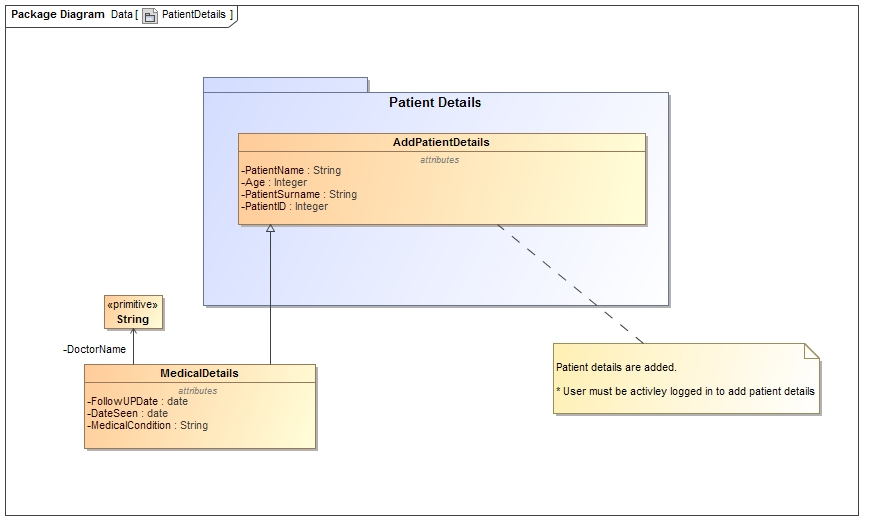
\includegraphics[width=1\linewidth]{./Graphics/addPatient}





%--------previewForm---------
\subsection{previewForm}
\textbf{Description:}
This use case allows the user to preview the form he has filled in before it is submitted
\subsubsection{Prioritization:}
Important
\subsubsection{Conditions and Data Structures:}
\textbf{Pre-Conditions:}
\begin{itemize}
	\item Form must have been completed.
\end{itemize}

\textbf{Post-Conditions:}
\begin{itemize}
	\item Display preview of patient's form before submission.
\end{itemize}
 
\subsubsection{Service Construct:}
